\documentclass{article}
\usepackage{amsmath, amssymb, amsthm}
\usepackage{physics}
\usepackage{float, subcaption, graphicx}
\usepackage{hyperref}

\title{Data-Driven Modeling of Landau Damping by Physics-Informed Neural Networks}
\author{Hunt Feng}
\date{\today}
\begin{document}
    \maketitle

    \begin{abstract}
        In this report, we successfully simulate the Landau damping using finite difference algorithm. The physics-informed neural network (PINN) is constructed. The PINN prediction for the first two time steps is good.
    \end{abstract}

    \section{Introduction}
    The fluid description of plasma is widely used today to mitigate the computational cost of kinetic models. It is derived by taking the velocity moments of the kinetic Vlasov equation. However, one major difficulty in constructing the fluid closures in collisionless plasmas is that it typically requires very nontrivial physical and mathematical analysis applied to the specific regime. With the prosperity of Artificial Intelligence in the past decade, the question naturally arises: Can Machine Learning assists in completing the challenging task by exploring the simulation data.
    
    \section{Landau Damping}
    Consider a collisionless plasma in the absence of magnetic field, the dynamics of the plasma can be described by the particle distribution $f_s(\mathbf{x},\mathbf{v},t)$, where $s=\{electron, ion\}$ stands for species. The evolution of distribution function is governed by the Vlasov equation,
    \begin{equation} \label{eq:vlasov}
        \pdv{f_s}{t} + \mathbf{v}_s\cdot \grad_\mathbf{r} f_s + \frac{q_s}{m_s}\mathbf{E}\cdot\grad_\mathbf{v} f_s = 0
    \end{equation}
    where $\grad_\mathbf{r}=(\partial_x, \partial_y, \partial_z)$ and $\grad_\mathbf{v}=(\partial_{v_x}, \partial_{v_y}, \partial_{v_z})$. In this report, we consider one-dimensional model in $x-v_x$ space for convenience. 
    
    To complete the system, we introduce the Poisson equation for electric potential,
    \begin{equation} \label{eq:poisson}
        \laplacian\phi = -\rho/\epsilon_0
    \end{equation}
    For convenience, we set the vacuum permittivity $epsilon_0=1$, and the charge density $\rho$ is defined by,
    \begin{equation} \label{eq:charge_density}
        \rho = \sum_s q_sn_s
    \end{equation}
    where the number density $n_s(x,t)$ is defined as
    \begin{equation} \label{eq:number_density}
        n_s(x,t) = \int f_s(x,v_s,t) dv_s
    \end{equation}
    By Gauss's law, we can get electric field,
    \begin{equation}\label{eq:electric_field}
        E(x,t) = -\grad\phi
    \end{equation}
    Equations (\ref{eq:vlasov})-(\ref{eq:electric_field}) forms a complete PDE system. We can investigate the evolution of distribution $f_s(x,v_s,t)$.

    Starting from a plasma at equilibrium. We assume the ions are too heavy to move in a short period of time. Then two perturbation modes is given to the number density of electron. Then the initial number densities of ions and electrons are
    \begin{align} \label{eq:initial_conditions}
        n_e(x,t=0) &= n_0(1 + A_1\cos (k_1x) + A_2\cos (k_2x + \varphi)) \\
        n_i(x,t=0) &= n_0
    \end{align}
    where $n_0$ is the number density of each species at equilibrium. $k_1$ and $k_2$ are the wavenumbers of the two perturbation modes, $A_1$ and $A_2$ are their amplitudes, and $\varphi$ is a random phase.
    
    Using the initial setup parameters listed in Table.\ref{table:simulation_parameters}, we got the results as shown in Fig.\ref{fig:simulation_data}.
    \begin{table} [H]
        \centering
        \caption{Parameters of finite difference simulation.}
        \begin{tabular}{ccccc}
            \hline
            \hline
            $k_1$ & $k_2$ & $A_1$ & $A_2$ & $\varphi$ \\
            \hline
            0.6 & 1.2 & 0.05 & 0.4 & 0.38716 \\
            \hline
            \hline
        \end{tabular}
        \label{table:simulation_parameters}
    \end{table}
    
    \begin{figure} [H]
        \centering
        \begin{subfigure}[b]{0.5\textwidth}
            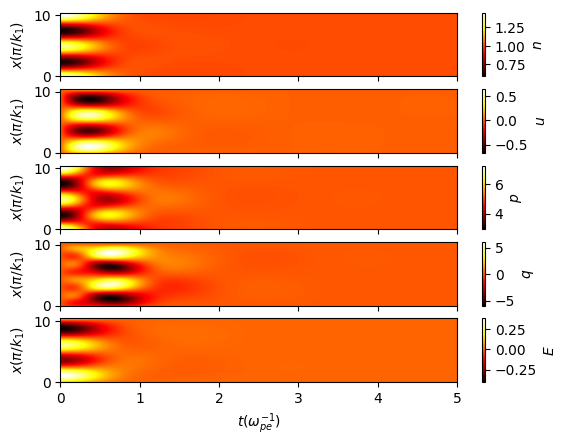
\includegraphics[width=\textwidth]{img/simulation_fields.png}    
        \end{subfigure}%
        \begin{subfigure}[b]{0.5\textwidth}
            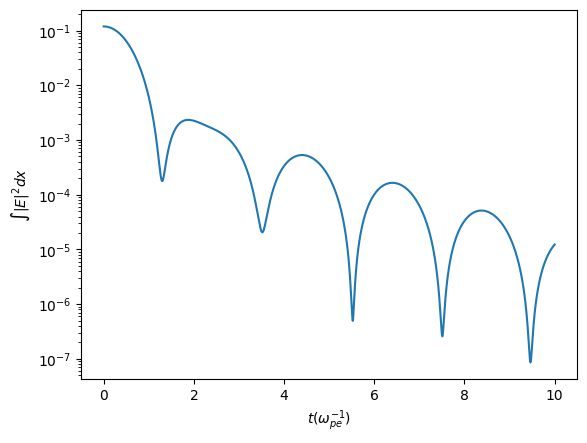
\includegraphics[width=\textwidth]{img/simulation_energy.png}    
        \end{subfigure}
        \caption{The simulation is run for 10 unit time in the region $\Omega=[0,2\pi/k_1]$}
        \label{fig:simulation_data}
    \end{figure}


    \section{Physics-Informed Neural network (PINN)}
    Physics-informed neural network is a type of neural network which embeds physical information. The loss function of PINN consists of residuals to the PDE system which governs the physics. \cite{qin_data-driven_2022} See part C of Fig.(\ref{fig:pinn_architecture}).

    \begin{figure} [H]
        \centering
        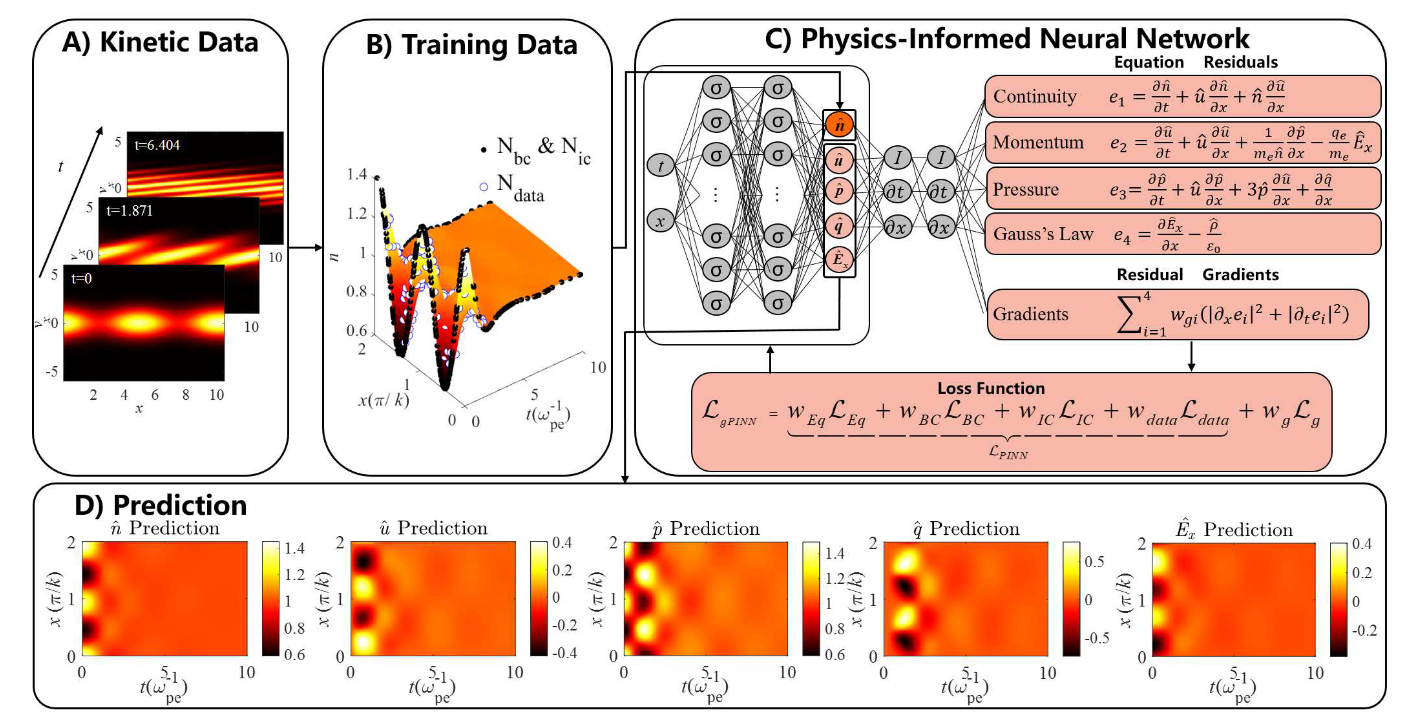
\includegraphics[width=\textwidth]{img/pinn_architecture.png}
        \caption{Physics-informed neural network (PINN) architecture for the multi-moment fluid model with an implicit fluid closure learned from the kinetic simulation data. The whole procedure includes A) kinetic simulation data generation, B) sparse sampling of training data, C) PINN construction with the constraints of different moment equation residuals and their gradients, and D) parameter prediction.}
        \label{fig:pinn_architecture}
    \end{figure}

    \section{Methodology}
    \subsection{Data preparation}
    The PINN as a parametric function approximator can be represented by a nonlinear function:
    \begin{equation} \label{eq:approximator}
        \hat{n},\hat{u},\hat{p},\hat{q},\hat{E} = \hat{\mathbf{F}}(t,x,\mathbf{\theta})
    \end{equation}
    where $\mathbf{\theta}=\{\mathbf{W,b}\}$ is the weight matrix and the bias vector of the neural network.

    This means for each input in the array $\{t_n,x_n\}_{n\geq0}$, the PINN produces an array of length 5, with each number corresponding to $\hat{n}(t_n,x_n)$,$\hat{u}(t_n,x_n)$, $\hat{p}(t_n,x_n)$, $\hat{q}(t_n,x_n)$, $\hat{E}(t_n,x_n)$.

    We will use the finite-difference simulation data as our training and testing dataset. 

    \subsection{Construction of loss function}
    The physical partial differential equation (PDE) residuals are incorporated into the loss function of the neural network as regularization, transforming the process of solving PDEs into an optimization problem by constraining the space of permissible solutions.

    We want the neural network to learn the closure relation to the fluid description of plasma
    \begin{equation} \label{eq:fluid_equations}
        \begin{aligned}
            \pdv{n}{t} + u\pdv{n}{x} + n\pdv{u}{x} &= 0 \\
            \pdv{u}{t} + u\pdv{u}{x} + \frac{1}{m_en}\pdv{p}{x} - \frac{q_e}{m_e}E &= 0 \\
            \pdv{p}{t} + u\pdv{p}{x} + 3p\pdv{u}{x} + \pdv{q}{x} &= 0 \\
            \pdv{E}{x} &= \frac{\rho}{\epsilon_0}
        \end{aligned}
    \end{equation}
    The first equation is the continuity equation for number density, the second equation describes the conservation of momentum of the plasma, the third one is the conservation of pressure. The last one is the Gauss's law. We see that the fluid description involves higher and higher velocity moments of the particle distribution. To close the system, we must need a closure relation. 

    The loss function is defined as
    \begin{equation} \label{eq:loss_funciton}
        L_{PINN} = w_{eq}L_{eq} + w_{bc}L_{bc} + w_{ic}L_{ic} + w_{data}L_{data}
    \end{equation}
    where $w_{eq}, w_{bc}, w_{ic}$ and $w_{data}$ are the weights of each loss function respectively. In this study, we choose the weights $w_{eq}=w_{bc}=w_{ic}=w_{data}=1$. In particular, we seek to minimize the residuals of the fluid moment equations, 
    \begin{equation} \label{eq:pde_residuals}
        \begin{aligned}
            e_1 &= \pdv{\hat{n}}{t} + \hat{u}\pdv{\hat{n}}{x} + \hat{n}\pdv{\hat{u}}{x} \\
            e_2 &= \pdv{\hat{u}}{t} + \hat{u}\pdv{\hat{u}}{x} + \frac{1}{m_e\hat{n}}\pdv{\hat{p}}{x} - \frac{q_e}{m_e}\hat{E} \\
            e_3 &= \pdv{\hat{p}}{t} + \hat{u}\pdv{\hat{p}}{x} + 3\hat{p}\pdv{\hat{u}}{x} + \pdv{\hat{q}}{x} \\
            e_4 &= \pdv{\hat{E}}{x} - \frac{\hat{\rho}}{\epsilon_0}
        \end{aligned}
    \end{equation}
    \begin{equation} \label{eq:loss_eq}
        L_{eq} = \frac{1}{N_{eq}} \sum_{j=1}^{N_{eq}}\sum_{i=1}^{4} \abs{e_i(t_j,x_j)}^2, t_j\in[0,T], x_j\in\Omega
    \end{equation}

    Here $e_1$ denotes the continuity equation residual, $e_2$ the momentum equation residual, $e_3$ the pressure equation residual, and $e_4$ the Gauss's law equation residual. $N_{eq}$ is the number of the trained data for $L_{eq}$. By minimizing the residuals to the fluid equations Eq.(\ref{eq:pde_residuals}), the neural networks "learns" the closure relation to the fluid equations, given the boundary conditions and initial conditions are known and sparsely sampled,

    \begin{equation} \label{eq:loss_bc}
        L_{bc} = \frac{1}{N_{bc}} \sum_{j=1}^{N_{bc}}\sum_{i=1}^{5} \abs{\hat{\mathbf{F}}(t_j,x_j)-\mathbf{F}(t_j,x_j)}^2, t_j\in[0,T], x_j\in\partial\Omega 
    \end{equation}
    \begin{equation} \label{eq:loss_ic}
        L_{ic} = \frac{1}{N_{ic}} \sum_{j=1}^{N_{ic}}\sum_{i=1}^{5} \abs{\hat{\mathbf{F}}(t_j,x_j)-\mathbf{F}(t_j,x_j)}^2, t_j=0, x_j\in\Omega
    \end{equation}

    Lastly, we sampled the number density in the first few time steps.
    \begin{equation} \label{eq:loss_data}
        L_{data} = \frac{1}{N_{data}} \sum_{j=1}^{N_{data}}\abs{\hat{n}(t_j,x_j)-n(t_j,x_j)}^2, t_j\in[0,T/5], x_j\in\Omega
    \end{equation}

    When computing the loss function, we can take advantage of the automatic differentiation in neural network.

    \subsection{Construction of PINN}
    The PINN consists of 5 hidden layers with 50 neurons in each layer. The activation function is Swish. The optimizer is chosen to be Adam with constant learning rate 0.01. The batch size in each training epoch is 10000. Finally, 10000 epochs were ran.

    \begin{table}
        \centering
        \caption{Summary of PINN parameters.}
        \begin{tabular}{ccc}
            \hline
            \hline
            Hidden layers, and No. of neurons & Optimizer &  Activation function  \\
            \hline
            5 and 50 & Adam &  Swish  \\
            \hline
            \hline
            Learning rate & Batch size & Epochs \\
            \hline
            0.01 & 10000 & 10000 \\
            \hline
            \hline
        \end{tabular}
    \end{table}

    \section{Result}
    \begin{figure} [H]
        \centering
        \begin{subfigure}[b]{0.5\textwidth}
            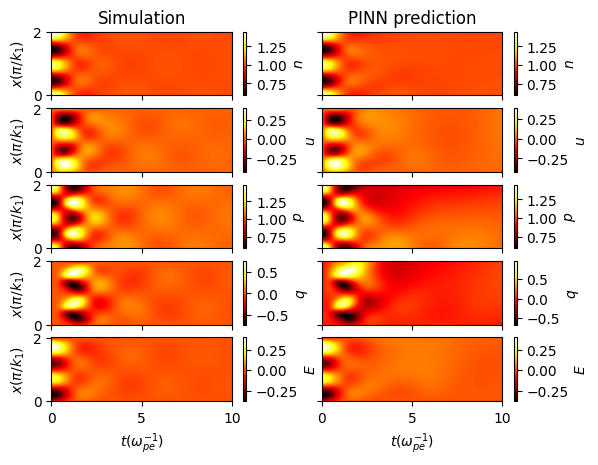
\includegraphics[width=\textwidth]{img/fields.png}
        \end{subfigure}%
        \begin{subfigure}[b]{0.5\textwidth}
            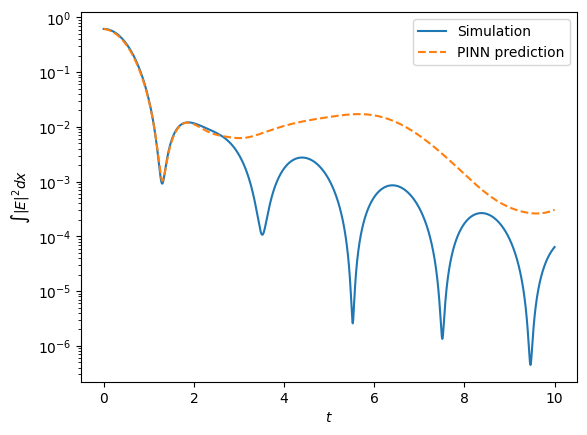
\includegraphics[width=\textwidth]{img/energy.png}
        \end{subfigure}
    \end{figure}
    The first two time step of the PINN prediction is good.

    \section{Conclusions and Discussions}
    By embedding the fluid equations Eq.(\ref{eq:fluid_equations}) into the loss function, the physical information is incorporated into the neural network. Minimizing the loss function, the neural network learns the closure relation to Eq.(\ref{eq:fluid_equations}). The PINN prediction is good in the first two time steps.

    According to the paper, we can improve the accuracy of PINN by introducing one more component to the loss function
    \begin{equation} \label{eq:loss_funciton}
        L_{gPINN} = w_{eq}L_{eq} + w_{bc}L_{bc} + w_{ic}L_{ic} + w_{data}L_{data} + \mathbf{w}_gL_{g}
    \end{equation}
    where
    \begin{equation} \label{eq:loss_g}
        \mathbf{w}_gL_{g} = \frac{1}{N_{g}} \sum_{j=1}^{N_{g}}\sum_{i=1}^{4} w_{g_i}\left(\abs{\pdv*{t}e_i(t_j,x_j)}^2 + \abs{\pdv*{x}e_i(t_j,x_j)}^2\right), t_j\in[0,T], x_j\in\Omega
    \end{equation}
    The $\mathbf{w}_g = \{w_{g_1}, w_{g_2}, w_{g_3}, w_{g_4}\}$ is an extra hyper-parameter in the gPINN architecture for optimization.

    \bibliography{references}
    \bibliographystyle{plain}
\end{document}